\chapter{Example chapter}
\label{chap:ex-ch}

This is an example chapter. 
\section{Math and formulae}
For inline math use \(t_hi^s\) or $t_{hi}s$ ---the recommended option is the first one---.
Inline math should be used for short expressions
or when referring to functions, \(f(x)\) or variable names like $x$.

For unnumberd equations use
\[
\mathcal{S} = \int_{t_0}^{t_1} \mathcal{L} \dd{t}
\]

and

\begin{equation*}
\var \mathcal{S} = 0.
\end{equation*}

For numbered equations use
\begin{equation}
\label{eq:time-evolution-heisenberg}
i \hbar \dv{A_H(t)}{t} = \comm{A_H(t)}{H}.
\end{equation}

\subsection{Details}

If you use a label for something, like an equation, you can reffer to it later in text, see eq.~\eqref{eq:time-evolution-heisenberg}.
For more details regarding the Heisenberg picture of Quantum Mechanics, see~\cite{Dirac1967, Sakurai2011} and also the
lecture notes~\cite{Baran, Zus}. Equation~\eqref{eq:time-evolution-heisenberg} reminds us of Hamilton's equations
\begin{align*}
  \dot{q}_k = [q_k,H], && \dot{p}_k = [p_k,H].
\end{align*}

An other important picture of Quantum Mechanics is the Schrödinger one. In this formulation the observables are time
independent and the states are evolving in time. The time evolution is given by the well-known Schrödinger equation
\[
  i \hbar \pdv{t} \ket{\Psi} = H \ket{\Psi}.
\]

If you have a very long formula, you can split it like this
\begin{equation}
\label{eq:long}
\begin{split}
\left(1+x\right)^n  &=  1 + nx + \frac{n\left(n-1\right)}{2!}x^2 \\
 &+ \frac{n\left(n-1\right)\left(n-2\right)}{3!}x^3 \\
 &+ \frac{n\left(n-1\right)\left(n-2\right)\left(n-3\right)}{4!}x^4 \\
 &+ \ldots
\end{split}
\end{equation}

\subsubsection{Definitions and theorems}

\begin{def*}[Joint probability]
Given two events $A$ and $B$, their joint probability, \(P(A \cap B)\), is the probability of the two events to occur simultaneously.
\end{def*}

\begin{theorem*}[Pythagorean theorem]
    	This is a theorem about right triangles and can be summarised in the next equation 
\[
	x^2 + y^2 = z^2
\]
\end{theorem*}

\section{Tables}

\begin{table}[ht]
\centering
\caption{Angular momentum}
\label{tab:my-label}
\begin{tabular}{llll}
\toprule
Type & Commutation relations & Eigenvalues & \\
\midrule
General & \(\comm{J_i}{J_j} = i \hbar \varepsilon_{ijk} J_k\)  & \(\vec{J}^2 \ket{jm} = j(j+1) \hbar^2 \ket{jm}\) & \(J_z \ket{jm} = m \hbar \ket{jm}\) \\ 
Orbital  & \(\comm{L_i}{L_j} = i \hbar \varepsilon_{ijk} L_k\)  & \(\vec{L}^2 \ket{lm} = l(l+1) \hbar^2 \ket{lm}\) & \(L_z \ket{lm} = m \hbar \ket{lm}\) \\
Spin  & \(\comm{S_i}{S_j} = i \hbar \varepsilon_{ijk} S_k\)  & \(\vec{S}^2 \ket{sm} = s(s+1) \hbar^2 \ket{sm}\) & \(S_z \ket{sm} = m \hbar \ket{sm}\) \\
\bottomrule
\end{tabular}
\end{table}

\section{Figures}

Figure~\ref{fig:parabolic} shows a simple figure. Two figures side by side in fig.~\ref{fig:hyperbolic}.

\begin{figure}[H]
  \centering
  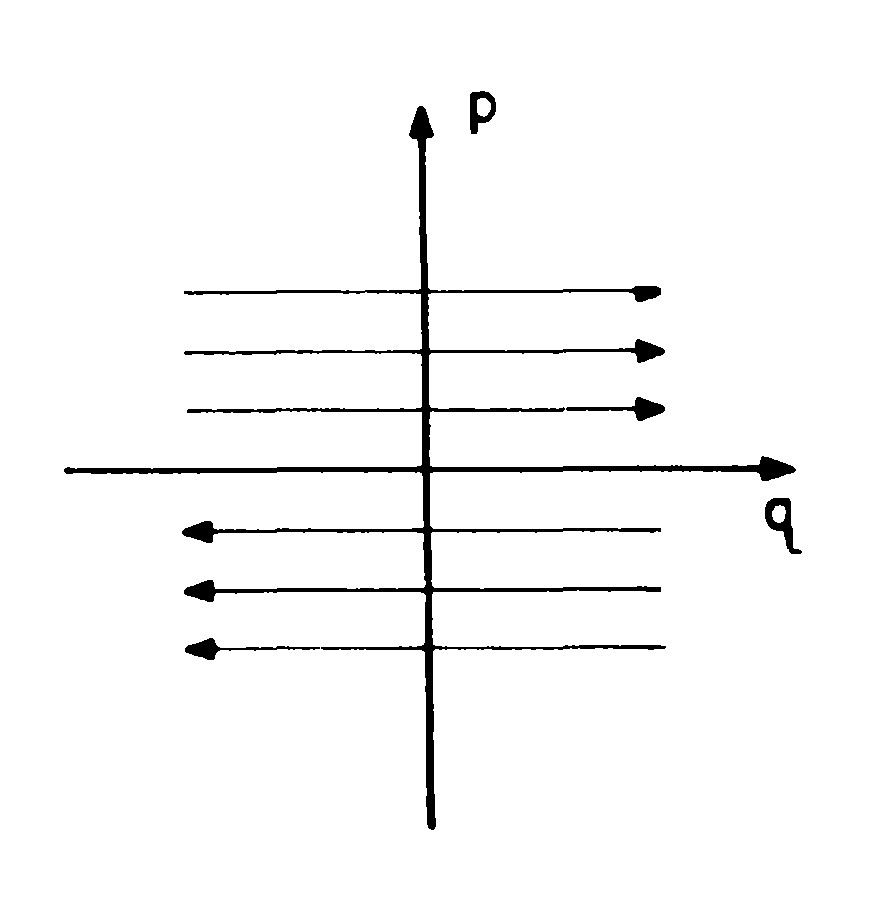
\includegraphics{parabolic}
  \caption{Parabolic fixed point}
\label{fig:parabolic}
\end{figure}

\begin{figure}[ht]
  \centering
  \begin{subfigure}[t]{0.45\textwidth}
    \centering
    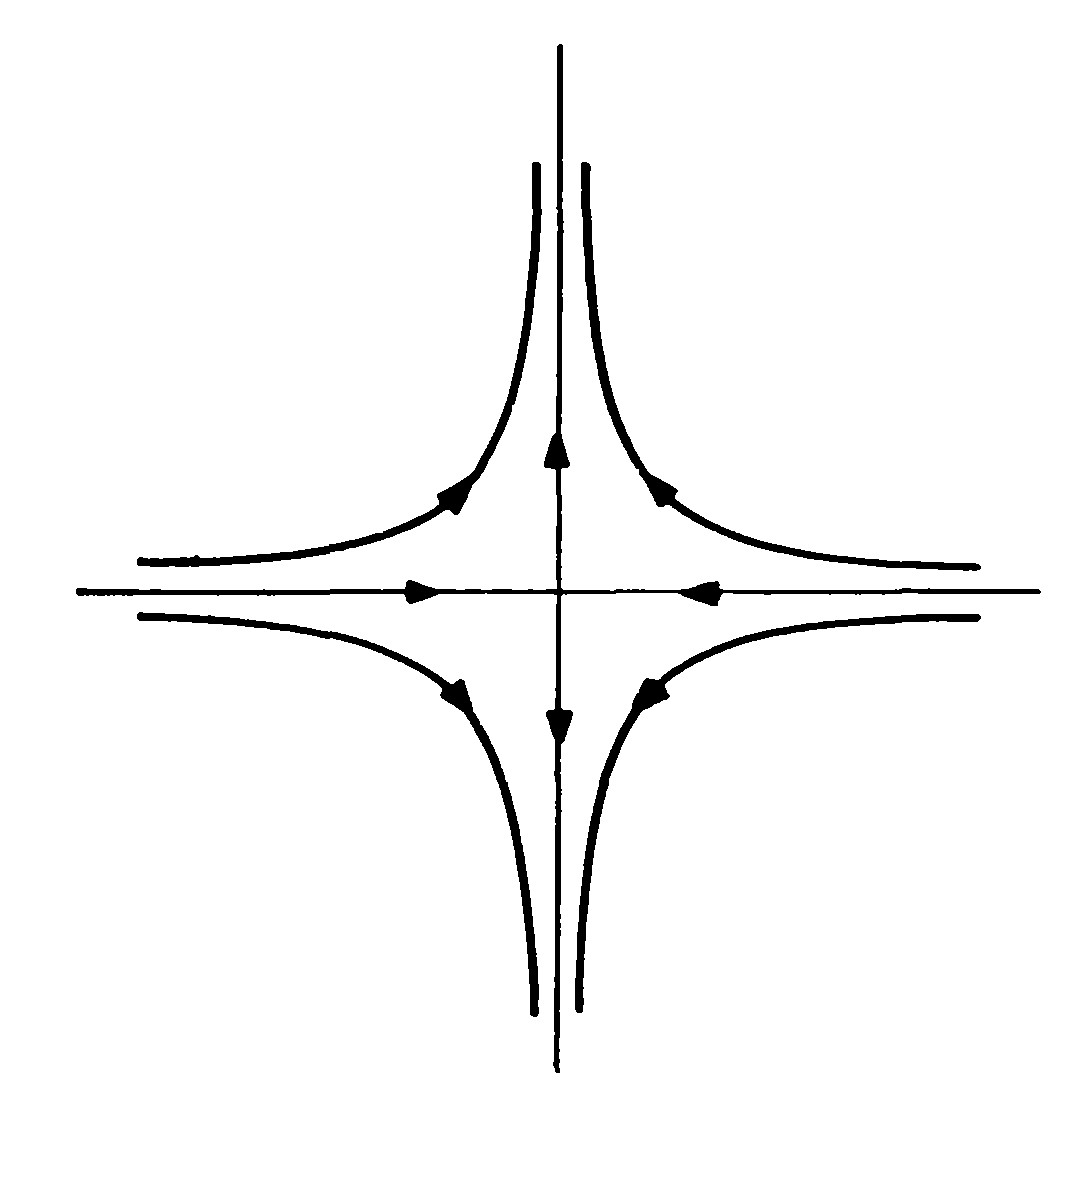
\includegraphics{hyperbolic}
    \caption{Hyperbolic fixed point}
  \end{subfigure}
~
  \begin{subfigure}[t]{0.45\textwidth}
    \centering
    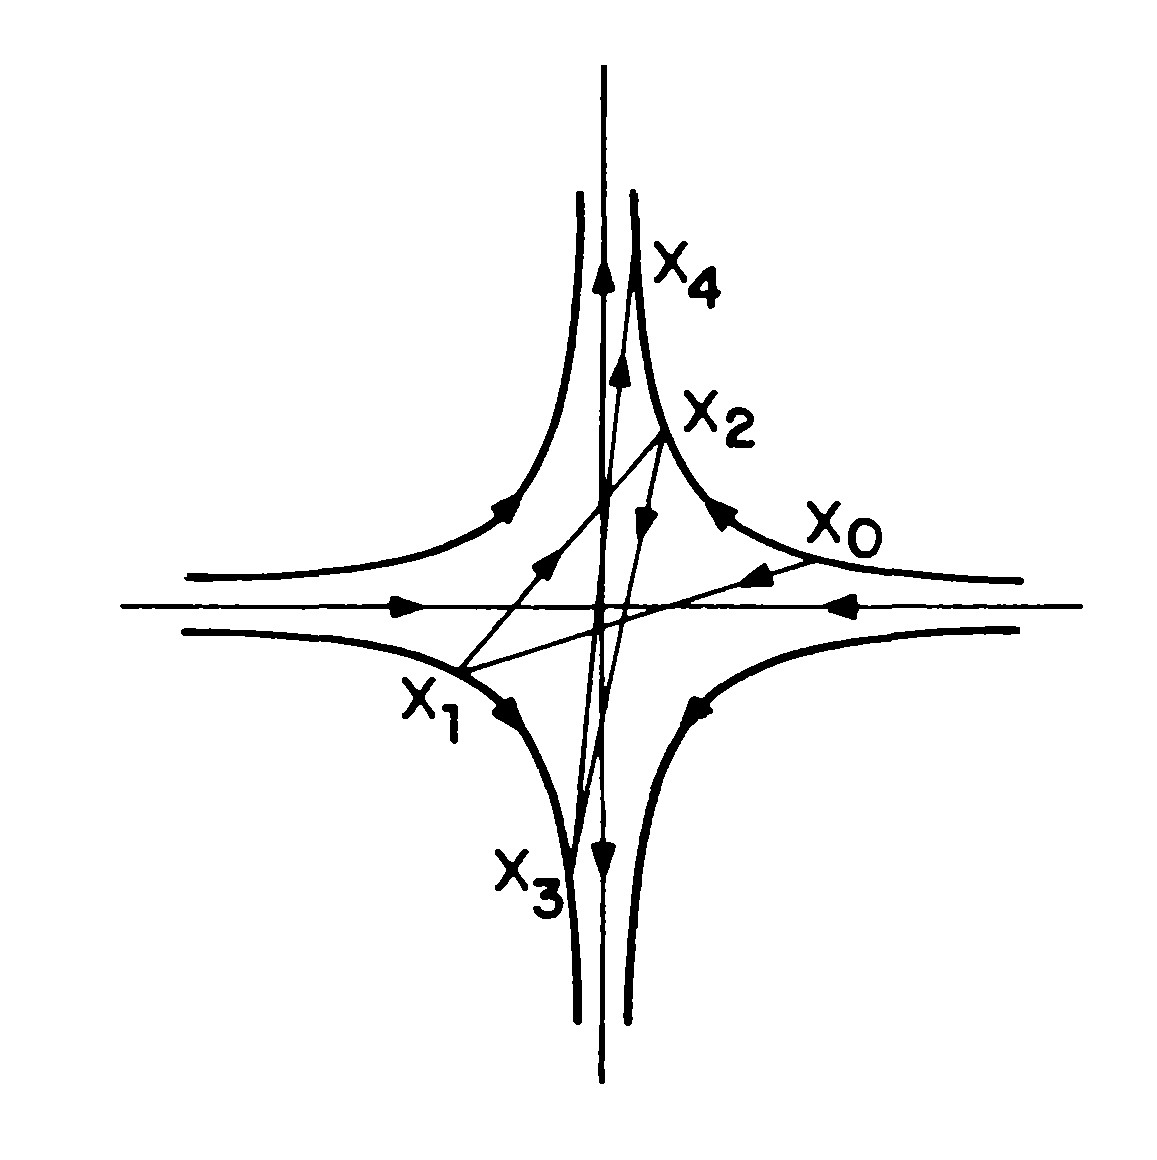
\includegraphics{hyperbolic-reflection}
    \caption{Hyperbolic-with-reflection fixed point}
  \end{subfigure}
\caption{}
\label{fig:hyperbolic}
\end{figure}



